\chapter{LİTERATÜR, KURAMSAL TEMEL VE ARAŞTIRMA BOŞLUĞU}
\label{chap:literatur}

Giriş bölümünde tezin ana savı, düşük güçteki verim--harmonik ödünleşimi ile aynı T-tipi donanımın enerji depolama işlevlerinde yeniden kullanılması olarak iki eksende tanımlanmıştı. Literatür bölümü, iki ekseni taşıyan dört bilgi alanını inceleyerek araştırma boşluğunu belirlemektedir: enerji depolama sistemlerinde güç dönüşüm mimarileri, üç seviyeli T-tipi dönüştürücünün kuramsal temeli, fotovoltaik çalışma profili ile kısmi yük performansı ve şebeke akım kontrolündeki ileri besleme yaklaşımları.

\section{Enerji Depolama Sistemlerinde Güç Dönüşüm Mimarileri}

Enerji depolama sistemleri, elektrik enerjisinin farklı zaman ölçeklerinde depolanmasını ve yeniden kullanılmasını sağlayan çok bileşenli yapılardır. Elektrokimyasal depolamanın yaygınlaşmasıyla birlikte batarya grubu, güç dönüşüm sistemi, batarya yönetim sistemi (Battery Management System, BYS), enerji yönetim sistemi, koruma ve ısıl yönetim birimleri aynı sistem sınırı içinde değerlendirilmeye başlanmıştır \citep{Chen2009,Aneke2016,Hannan2017}. Güç dönüşüm sistemi, bataryanın değişken doğru gerilimi ile şebeke veya yük arasındaki çift yönlü enerji akışını düzenlerken BYS hücre gerilimlerini, sıcaklıkları ve şarj durumunu izleyerek güvenli çalışma sınırlarını korur \citep{Plett2015,Khan2024}. Dönüştürücü ve BYS işlevleri fiziksel olarak ayrı olsa bile enerji akışı, güvenlik ve kullanılabilir kapasite bakımından birbirine bağımlıdır.

Tipik bir şebeke bağlantılı EDS'nin güç ve bilgi akışları Şekil~\ref{fig:eds-mimarisi} üzerinde özetlenmiştir. Kesintisiz çizgiler güç aktarım yolunu, kesikli çizgiler ise ölçüm ve yönetim bağlantılarını göstermektedir.

\begin{figure}[htbp]
  \centering
  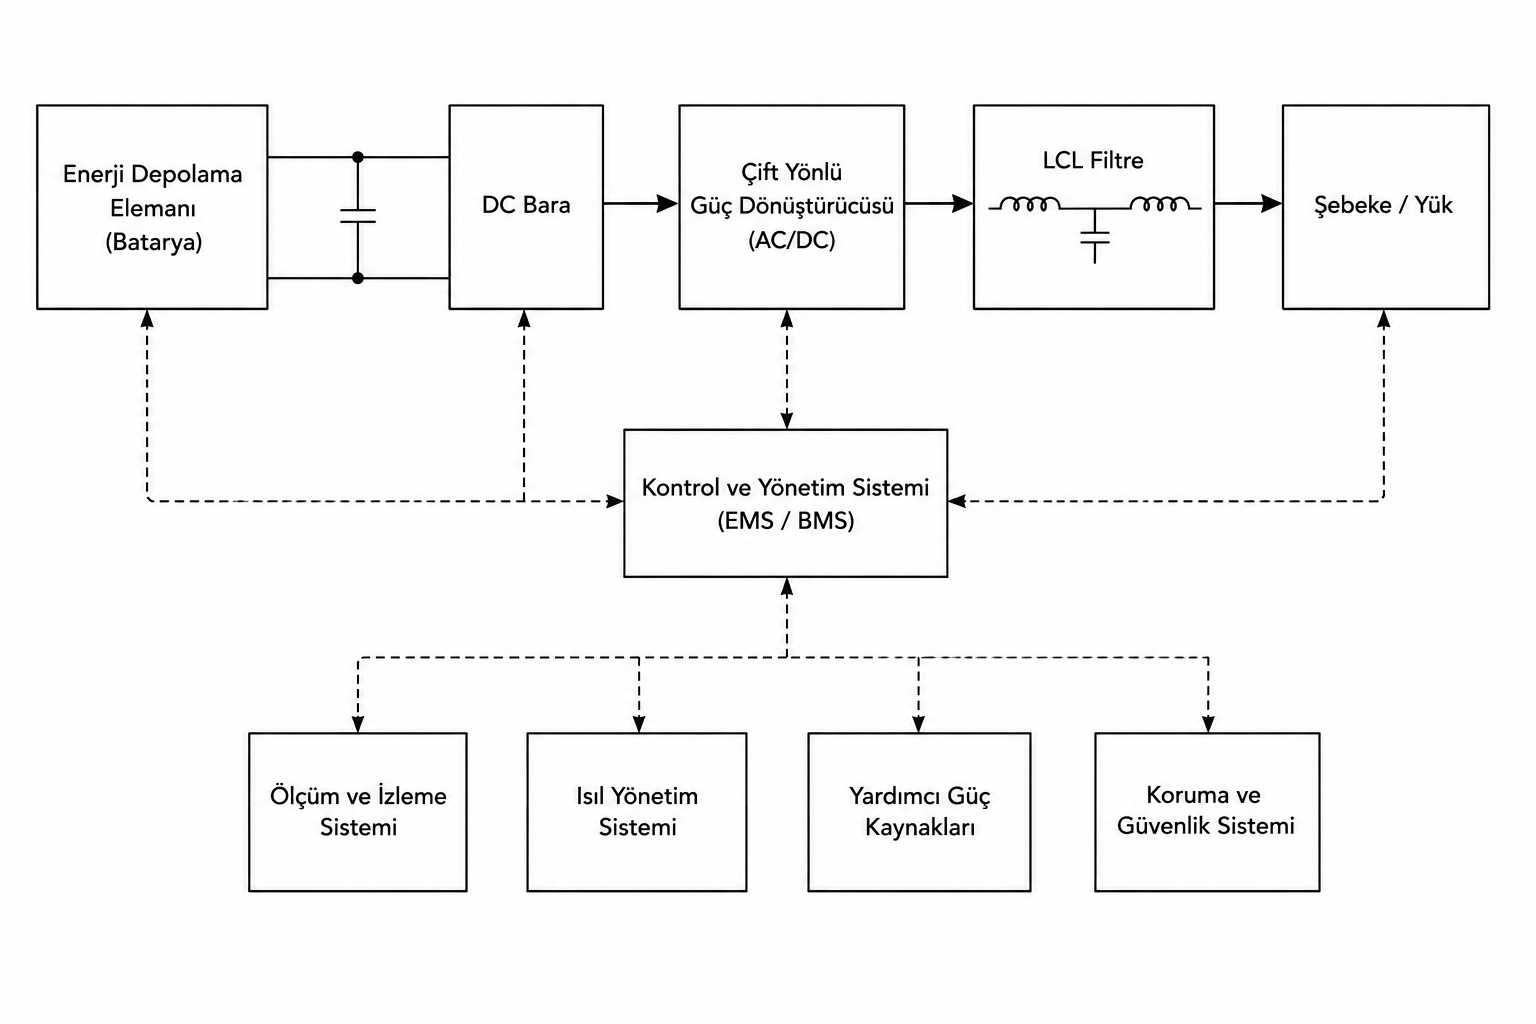
\includegraphics[width=0.96\textwidth]{literatur/gecici_eds_mimarisi_eski_tez.png}
  \caption{Şebeke bağlantılı bir enerji depolama sisteminin temel bileşenleri ve bilgi akışları.}
  \label{fig:eds-mimarisi}
\end{figure}

Geleneksel şebeke bağlantılı bir EDS'de batarya ile DA bara arasında çift yönlü DA/DA dönüştürücü, DA bara ile şebeke arasında evirici/doğrultucu ve hücreler arasında ayrı bir dengeleme devresi bulunabilir. Katların ayrılması, her işlev için bağımsız tasarım ve koruma olanağı sunar; karşılığında yarı iletken, manyetik eleman, sürücü, algılayıcı ve soğutma gereksinimini artırır. Sistem maliyeti çalışmalarında batarya paketi baskın kalem olsa da güç elektroniği donanımının maliyet, kayıp ve hacim üzerindeki etkisi ihmal edilemez \citep{Ramasamy2023,Lazard2024}. İşlevlerin ortak elemanlarla gerçekleştirilmesi, özellikle şarj ve deşarj kiplerinin aynı anda etkin olmadığı uygulamalarda donanım kullanım oranını yükseltme potansiyeli taşır.

\begin{table}[htbp]
  \centering
  \caption{Enerji depolama sistemi bileşenlerinin toplam sistem maliyetindeki tipik pay aralıkları \citep{Ramasamy2023,Lazard2024}.}
  \label{tab:eds-maliyet-dagilimi}
  \begin{tabular}{>{\raggedright\arraybackslash}p{0.67\textwidth} c}
    \toprule
    \textbf{Sistem bileşeni} & \textbf{Maliyet payı (\%)} \\
    \midrule
    Batarya paketi & 50--70 \\
    Güç dönüştürücüleri (evirici, PFC ve DA/DA) & 10--20 \\
    Batarya yönetim sistemi & 3--8 \\
    Enerji yönetim sistemi & 2--5 \\
    Isıl yönetim ve soğutma & 3--10 \\
    Koruma ve güvenlik sistemleri & 2--5 \\
    Yardımcı güç kaynakları ve haberleşme & 1--3 \\
    Mekanik yapı ve kablolama & 5--10 \\
    \bottomrule
  \end{tabular}
\end{table}

Aralıkların toplamı tek bir tasarımı temsil etmediği için Tablo~\ref{tab:eds-maliyet-dagilimi} içindeki yüzde sütunu doğrudan toplanmamalıdır; her satır farklı proje, güç ve tedarik koşullarından türetilen tipik bir aralıktır. Tablo, tezin GT-tipi mimarisindeki eleman paylaşımının neden ekonomik olarak anlamlı bir araştırma sorusu olduğunu gösterir; tek başına maliyet azalımını kanıtlamaz.

Batarya paketinin kullanılabilir ömrü; deşarj derinliği, hücre gerilimi, sıcaklık, akım oranı ve hücreler arası dengesizlikten etkilenir \citep{Vetter2005,Smith2017,Chen2021,Feng2018}. Şekil~\ref{fig:batarya-omur-guvenlik} altındaki deşarj derinliği--çevrim ömrü eğrisi ile güvenli çalışma bölgesi, belirli bir hücre kimyasının veri sayfası yerine literatürden uyarlanmış temsilî ilişkileri gösterdiğinden tasarım sınırı olarak kullanılmamalıdır.

\begin{figure}[htbp]
  \centering
  \begin{subfigure}[t]{0.49\textwidth}
    \centering
    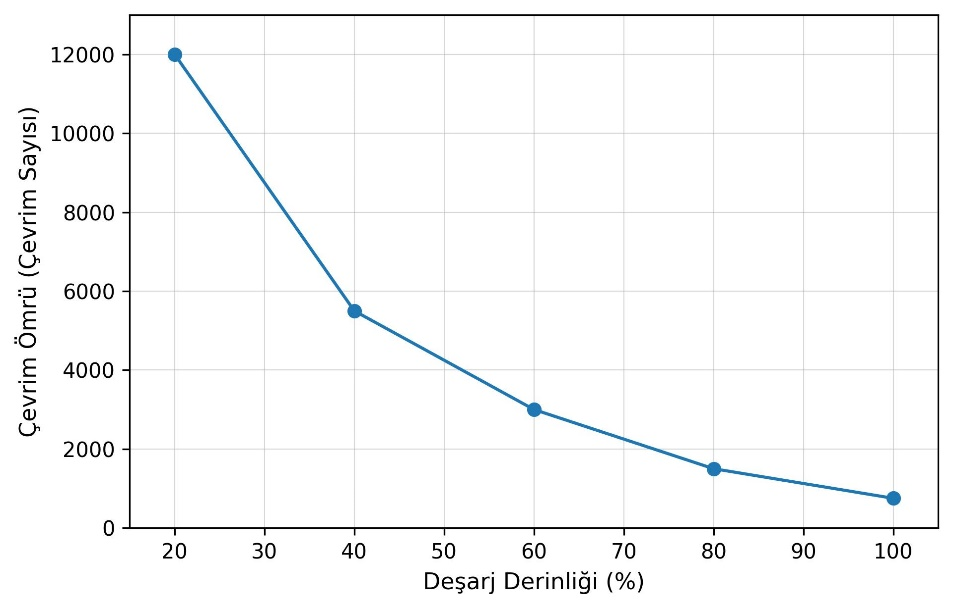
\includegraphics[width=\textwidth]{literatur/onceki_tez_dod_cevrim.jpg}
    \caption{Deşarj derinliği--çevrim ömrü ilişkisi.}
  \end{subfigure}\hfill
  \begin{subfigure}[t]{0.49\textwidth}
    \centering
    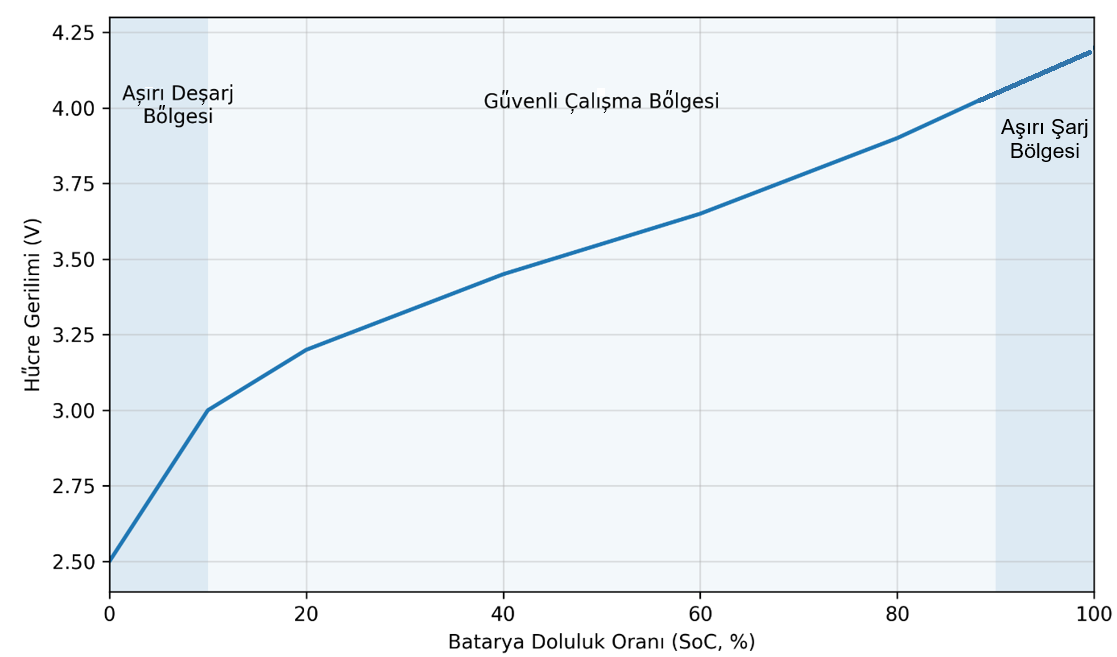
\includegraphics[width=\textwidth]{literatur/onceki_tez_guvenli_calisma.png}
    \caption{Temsilî gerilim ve doluluk sınırları.}
  \end{subfigure}
  \caption{Batarya ömrü ve güvenli işletim için kullanılan temsilî eğriler; \citet{Smith2017}, \citet{Chen2021} ve \citet{Feng2018} temel alınarak uyarlanmıştır.}
  \label{fig:batarya-omur-guvenlik}
\end{figure}

Hücre gerilimi, akım ve sıcaklık ölçümleri BYS denetleyicisine taşınır; koruma, kontaktör ve dengeleme komutları aynı karar katmanında üretilir. Tipik bir BYS'nin işlevsel mimarisi Şekil~\ref{fig:bys-mimarisi} üzerinde verilmiştir. Mimari, GT-tipi yapının hangi işlevleri ortak güç elemanlarına taşımayı hedeflediğini tanımlayan başvuru noktasıdır.

\begin{figure}[htbp]
  \centering
  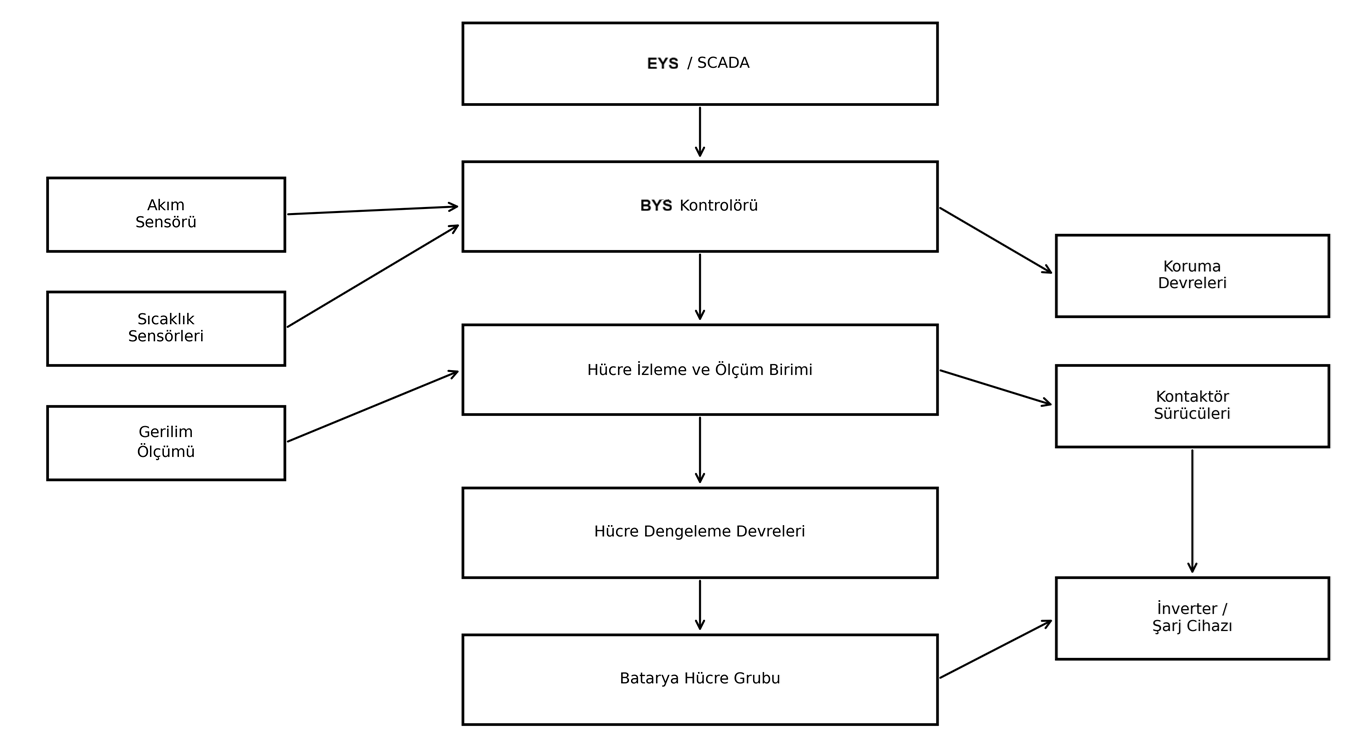
\includegraphics[width=0.94\textwidth]{literatur/onceki_tez_bys_mimarisi.png}
  \caption{Tipik bir batarya yönetim sisteminin ölçüm, karar, koruma ve dengeleme işlevleri.}
  \label{fig:bys-mimarisi}
\end{figure}

\begin{table}[htbp]
  \centering
  \caption{Geleneksel BYS ile hücre bazlı enerji yönetiminin işlevsel karşılaştırması.}
  \label{tab:bys-islev-karsilastirma}
  \setlength{\tabcolsep}{4pt}
  \begin{tabularx}{\textwidth}{>{\raggedright\arraybackslash}X >{\centering\arraybackslash}p{0.22\textwidth} >{\centering\arraybackslash}p{0.25\textwidth}}
    \toprule
    \textbf{İşlev} & \textbf{Geleneksel BYS} & \textbf{Hücre bazlı yönetim} \\
    \midrule
    Hücre izleme, koruma ve dengeleme & Var & Var \\
    Hücre bazlı şarj kontrolü & Sınırlı & Var \\
    Hücre bazlı deşarj kontrolü & Sınırlı & Var \\
    Ömür optimizasyonu & Dolaylı & Doğrudan \\
    \bottomrule
  \end{tabularx}
\end{table}

Tablo~\ref{tab:bys-islev-karsilastirma}'daki ``doğrudan'' ifadesi bir ömür kazancı yüzdesi değil, hücrenin güç yoluna ayrı ayrı müdahale edilebilmesini tanımlar. Sayısal ömür artışı ancak hücre kimyası, görev profili, sıcaklık ve yaşlanma testi birlikte verildiğinde ileri sürülebilir.

Seri bağlı hücre veya modüllerde kapasite, iç direnç, sıcaklık ve yaşlanma farklılıkları paket performansını en zayıf birimle sınırlandırabilir. Pasif dengeleme fazla enerjiyi dirençlerde harcarken aktif dengeleme kapasitör, endüktör, transformatör veya çift yönlü dönüştürücü üzerinden enerji aktarır \citep{Daowd2011,Khan2024}. Aktif yöntemler enerji kaybını azaltabilse de ilave anahtar ve manyetik eleman gereksinimi doğurur. Literatürdeki yeniden yapılandırılabilir batarya sistemleri, hücre veya modül bağlantılarını güç anahtarlarıyla değiştirerek dengeleme, arıza yalıtımı ve farklı terminal gerilimlerini aynı donanım üzerinden sağlamayı hedeflemektedir. Momayyezan ve arkadaşları, yüksek gerilimli batarya sisteminde yük besleme, geri kazanım, şarj ve modüller arası dengeleme kipleri için yarı iletkenleri ve bir endüktörü paylaşan bütünleşik bir dönüştürücü önermiş ve beş modüllü ölçekli prototiple çalışma kiplerini göstermiştir \citep{Momayyezan2016}. Farakhor ve arkadaşları ise yeniden yapılandırılabilir anahtar dizisini hücre düzeyindeki DA/DA dönüştürücülerle birleştirerek arızalı hücre yalıtımı, güç paylaşımı, şarj durumu ve sıcaklık dengelemesi sağlamış; yaklaşımı benzetim ve laboratuvar prototipiyle doğrulamıştır \citep{Farakhor2023}.

Pasif ve başlıca aktif dengeleme ailelerinin enerji aktarım elemanları Şekil~\ref{fig:dengeleme-yontemleri} üzerinde karşılaştırılmıştır. Şekil, yöntemlerin ayrıntılı devre tasarımından çok enerji yolundaki temel farkı göstermek amacıyla verilmiştir.

\begin{figure}[htbp]
  \centering
  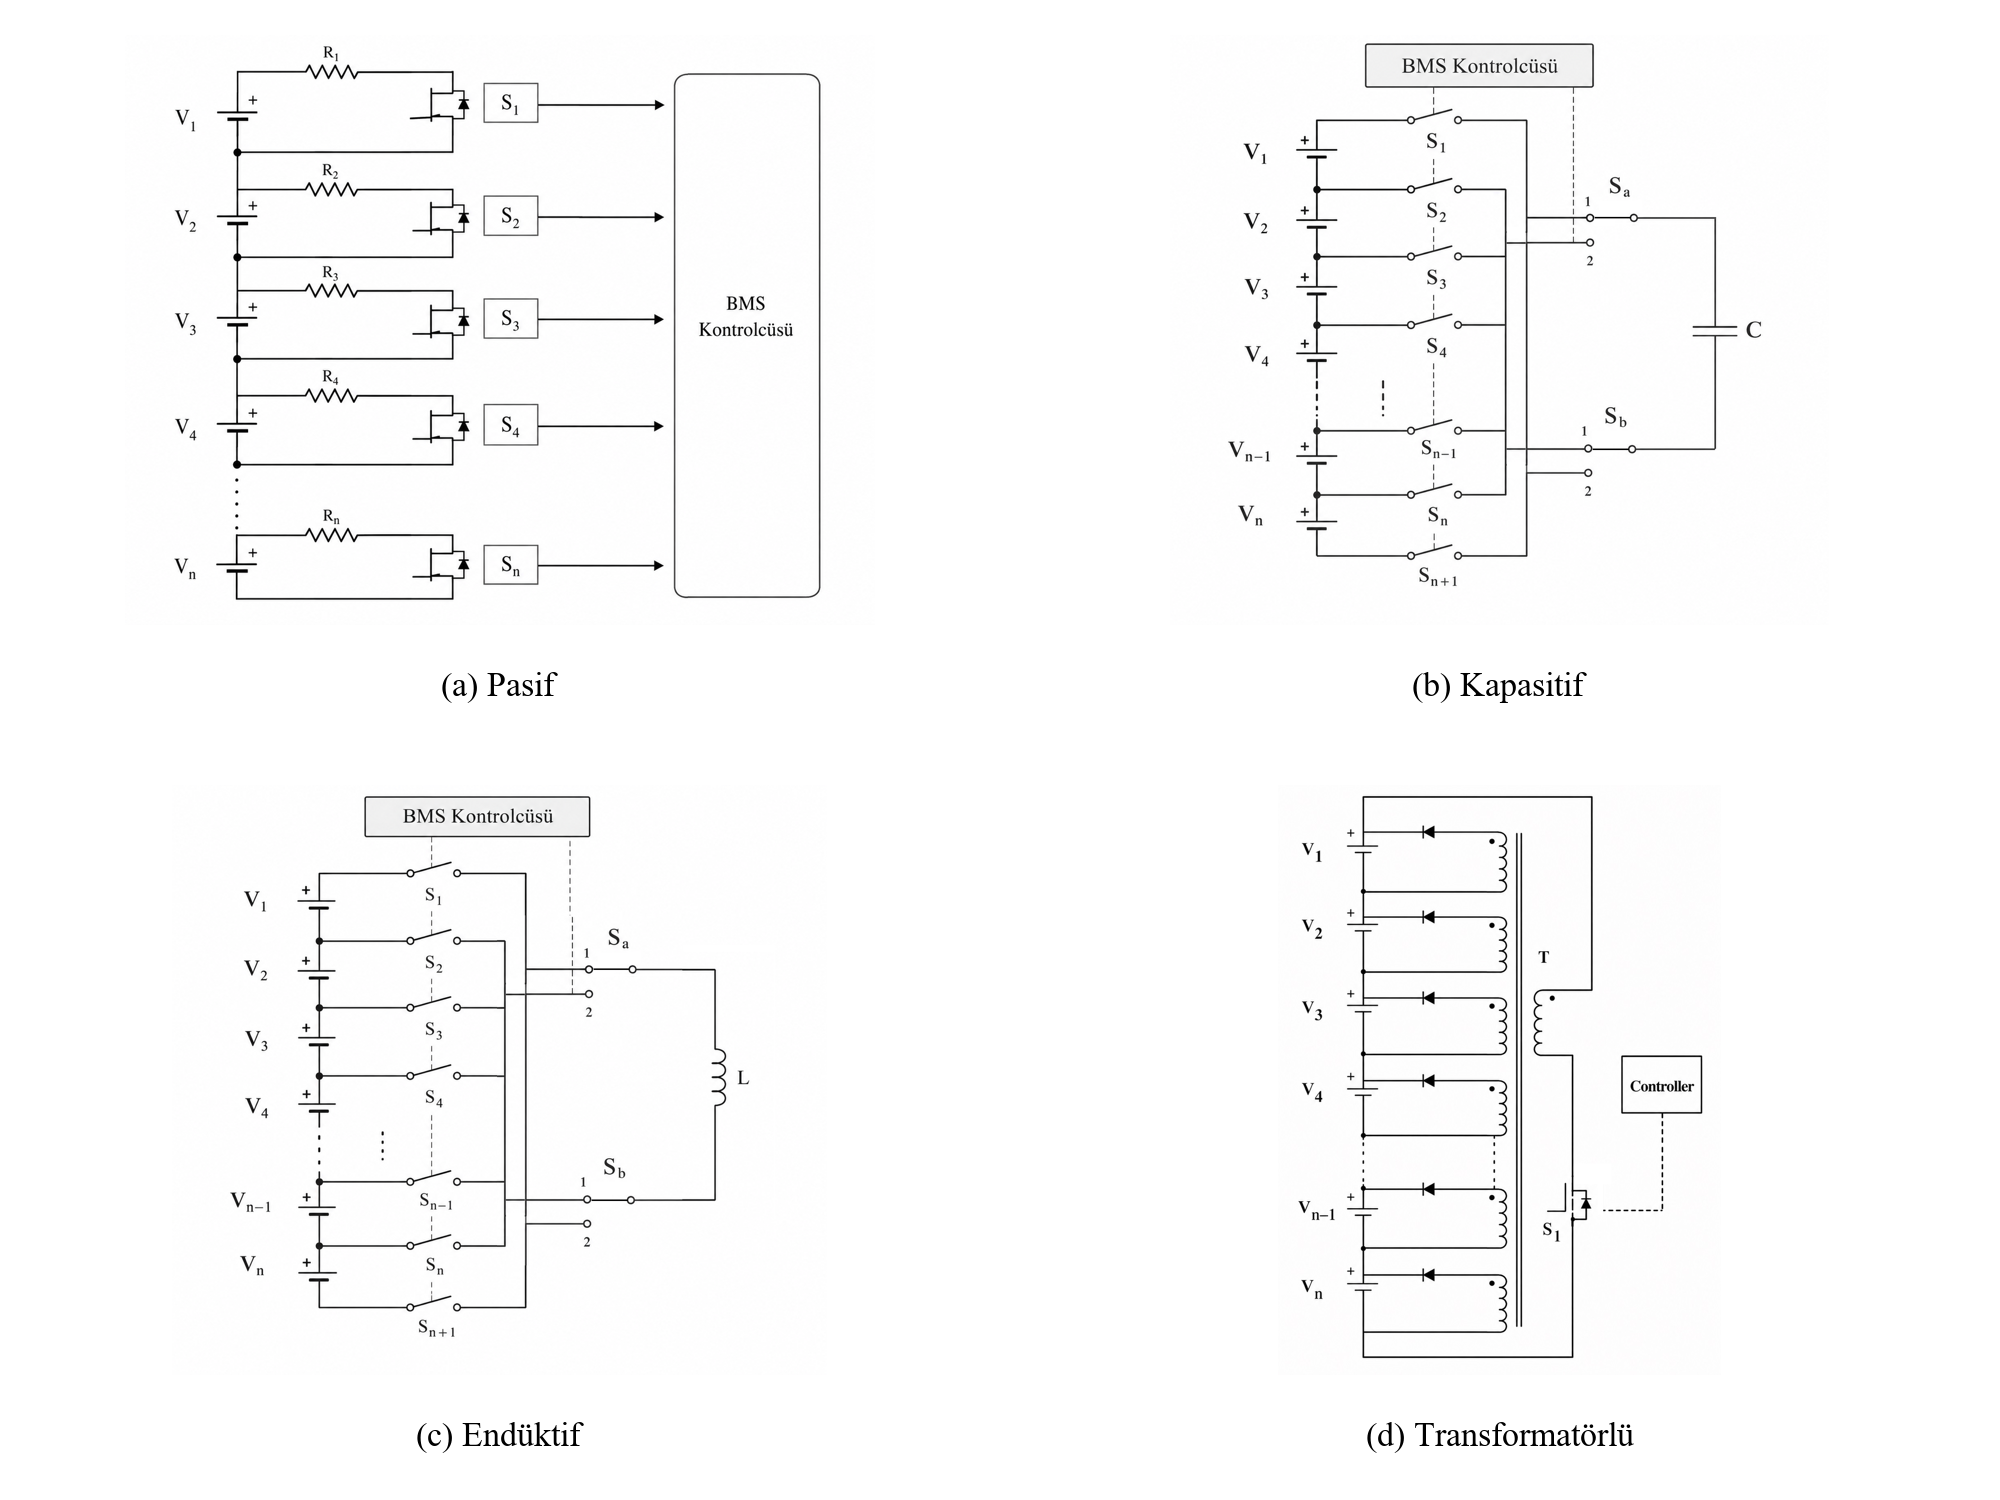
\includegraphics[width=0.94\textwidth]{literatur/gecici_dengeleme_yontemleri_bilesik.png}
  \caption{Pasif, kapasitif, endüktif ve transformatörlü hücre dengeleme yapılarının kavramsal karşılaştırması \citep{Daowd2011,Khan2024}.}
  \label{fig:dengeleme-yontemleri}
\end{figure}

Pasif dengeleme yönteminde, diğer hücrelere göre daha yüksek gerilim veya şarj durumuna sahip hücreye paralel bağlanan direnç üzerinden enerji harcanır. Anahtarın görev oranı hücreden çekilen dengeleme akımını belirler. Az sayıda eleman, basit denetim ve düşük maliyet başlıca avantajlardır. Fazla enerjinin ısıya dönüştürülmesi, soğutma gereksinimi ve düşük şarj durumundaki hücrelere enerji aktarılamaması ise yöntemin temel sınırlılıklarını oluşturur \citep{Daowd2011,Khan2024}.

Kapasitif dengelemede, anahtarlanan bir kapasitör farklı hücrelere sırasıyla bağlanarak gerilimi yüksek hücreden enerji alır ve gerilimi düşük hücreye aktarır. Manyetik eleman gerektirmeyen yapı, paketleme ve maliyet bakımından avantaj sağlayabilir. Dengeleme akımının hücreler arasındaki gerilim farkına bağlı olması, uzak hücreler arasında enerjinin birden fazla aktarım adımından geçmesi ve anahtar sayısının hücre sayısıyla artması dengeleme süresini uzatabilir \citep{Daowd2011,Khan2024}.

Endüktif dengeleme yönteminde enerji, anahtarlama sırasında bir endüktörde depolanır ve seçilen hücreye veya paket hattına kontrollü akım olarak aktarılır. Anahtarlama görev oranı üzerinden enerji akışının düzenlenebilmesi, kapasitif yönteme göre daha yüksek ve öngörülebilir dengeleme akımlarına olanak tanır. Endüktör, akım algılama, sürücü ve çift yönlü anahtarlama gereksinimleri devre ile denetim karmaşıklığını artırır \citep{Daowd2011,Khan2024}.

Transformatörlü yapılarda hücre sargıları ile ortak sargı arasındaki manyetik bağ; hücreden pakete, paketten hücreye veya seçilen hücreler arasında yalıtımlı enerji aktarımı sağlayabilir. Çoklu sargı yapısı farklı enerji yollarını desteklediği için hücre bazlı şarj ve deşarj işlevlerine geçiş bakımından önemlidir. Sargı sayısı, kaçak endüktans, sürme düzeni, hacim ve üretim maliyeti uygulama büyüdükçe belirleyici sınırlılıklara dönüşür \citep{Daowd2011,Khan2024}.

\begin{table}[htbp]
  \centering
  \caption{Başlıca hücre dengeleme ailelerinin nitel karşılaştırması \citep{Daowd2011,Khan2024}.}
  \label{tab:dengeleme-karsilastirma}
  \setlength{\tabcolsep}{3pt}
  \begin{tabularx}{\textwidth}{>{\raggedright\arraybackslash}p{0.20\textwidth} *{4}{>{\centering\arraybackslash}X}}
    \toprule
    \textbf{Yöntem} & \textbf{Enerji geri kazanımı} & \textbf{Maliyet} & \textbf{Karmaşıklık} & \textbf{Aktarım hızı} \\
    \midrule
    Pasif & Yok & Düşük & Düşük & Düşük \\
    Anahtarlamalı kapasitör & Var & Düşük--orta & Orta & Düşük--orta \\
    Endüktif & Var & Orta & Yüksek & Orta--yüksek \\
    Transformatörlü & Var & Yüksek & Yüksek & Uygulamaya bağlı \\
    \bottomrule
  \end{tabularx}
\end{table}

Nitel sınıflar topoloji, hücre sayısı ve dengeleme akımıyla değişebildiğinden Tablo~\ref{tab:dengeleme-karsilastirma} kesin bir sıralama değil, tasarım alanını özetleyen bir karşılaştırmadır. Dört yöntem birlikte değerlendirildiğinde tek bir dengeleme yapısının verim, hız, maliyet ve devre karmaşıklığı açısından her uygulamada üstün olmadığı görülür. Tezin GT-tipi mimari katkısı, dört dengeleme yönteminden birini genel olarak en iyi ilan etmek yerine, şarj--deşarj ve hücre yönetimi işlevlerinde mevcut yarı iletkenlerin yeniden görevlendirilmesine odaklanmaktadır. Şekil~\ref{fig:dengeleme-yontemleri}, ilerleyen bölümlerde sunulan işlev paylaşımının neden ayrı dengeleme donanımına alternatif oluşturabileceğini açıklayan kuramsal geçiş niteliğindedir.

Yeniden yapılandırılabilir sistemlerin esneklik kazancı yeni tasarım ödünleşimleri oluşturur. Anahtar sayısı yükseldikçe iletim kaybı, sürücü karmaşıklığı, yanlış anahtarlama riski ve güvenli kip geçişi gereksinimi büyür. Huang ve arkadaşlarının modüler yeniden yapılandırılabilir EDS çalışması, üç anahtarlı modül yapısıyla farklı bağlantıları ve arıza yalıtımını desteklerken işlev sayısı ile devre karmaşıklığı arasındaki ödünleşimi açıkça göstermiştir \citep{Huang2024}. Bütünleştirme, yalnızca eleman sayısını azaltma iddiasıyla değerlendirilemez; her çalışma kipi için akım yolu, eleman zorlanması, geçiş sırası, kayıp ve doğrulama düzeyi birlikte verilmelidir.

\section{Üç Seviyeli T-Tipi Dönüştürücünün Kuramsal Temeli}

EDS mimarisindeki güç dönüşüm katının verimi ve akım kalitesi, seçilen dönüştürücü topolojisine doğrudan bağlıdır; kesim, tezin odaklandığı T-tipi yapının literatürdeki yerini kurmaktadır. Gerilim kaynaklı iki seviyeli evirici, faz çıkışını DA baranın pozitif ve negatif uçları arasında anahtarlar. Yüksek anahtarlama frekansı akım dalgalanmasını ve filtre gereksinimini azaltırken anahtarlama kayıplarını artırır. Çok seviyeli dönüştürücüler, çıkış gerilimini daha küçük basamaklarla oluşturarak yarı iletken gerilim zorlanmasını, $dv/dt$ değerini ve filtreleme gereksinimini azaltmayı amaçlar \citep{Mohan2003,Holmes2003}. Üç seviyeli nötr nokta kenetlemeli (Neutral Point Clamped, NPC) yapı, sıfır seviyesini kenetleme diyotlarıyla üretirken T-tipi yapı nötr noktayı çift yönlü kontrollü bir anahtar kolu üzerinden faz çıkışına bağlar.

Bir T-tipi faz kolunda dış anahtarlar faz düğümünü DA baranın pozitif veya negatif yarısına, nötr anahtar çifti ise orta noktaya bağlar. İdeal anahtarlama durumları $+V_{\mathrm{dc}}/2$, $0$ ve $-V_{\mathrm{dc}}/2$ seviyelerini oluşturur. Pozitif ve negatif aktif durumlarda akım dış anahtarlar üzerinden, sıfır durumunda ise akım yönüne bağlı olarak nötr kol üzerinden akar. Nötr kol elemanlarının daha düşük gerilim sınıfında seçilebilmesi ile aktif durumdaki seri eleman sayısının NPC yapıya göre azalması, uygun gerilim ve anahtarlama frekansı aralığında iletim ve anahtarlama kayıpları açısından avantaj sağlayabilir.

T-tipi faz kolunun temel devre yapısı Şekil~\ref{fig:t-tipi-faz-kolu} üzerinde gösterilmiştir. Aynı devre, Bölüm~\ref{chap:sistem} içinde her anahtarlama durumu için akım yönleri işaretlenerek ayrıntılandırılacaktır.

\begin{figure}[htbp]
  \centering
  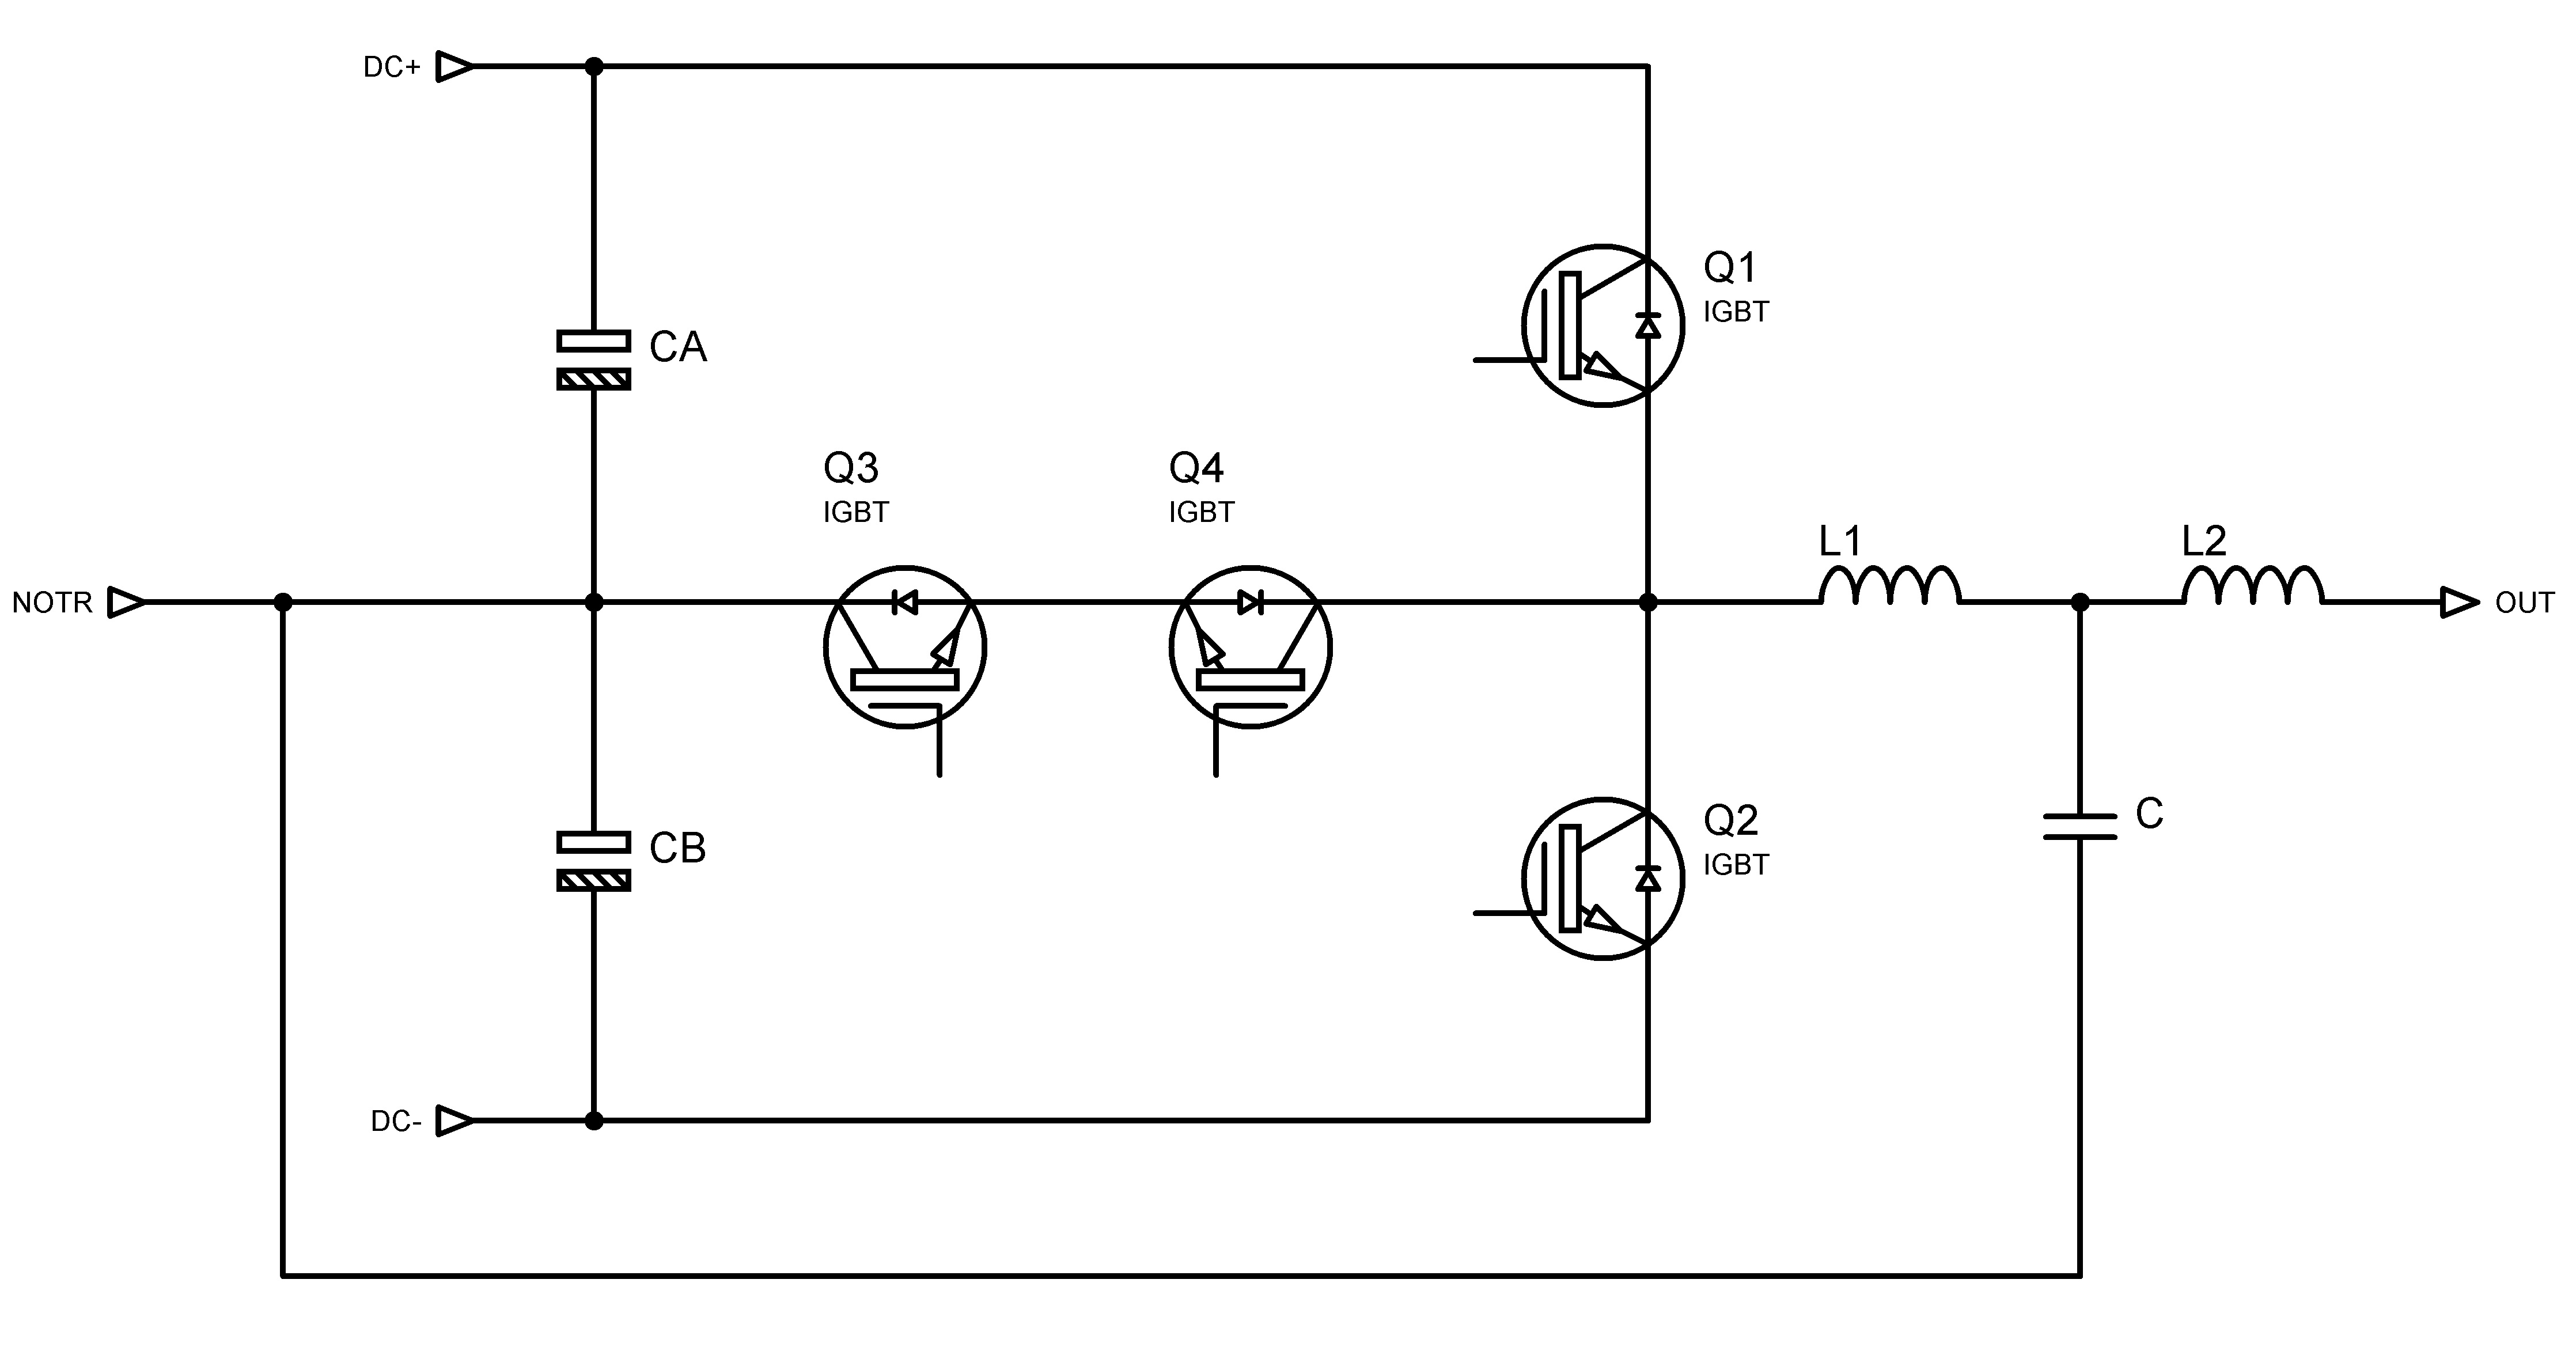
\includegraphics[width=0.88\textwidth]{literatur/gecici_t_tipi_faz_kolu_eski_tez.jpg}
  \caption{Üç seviyeli T-tipi eviricinin tek faz kolu ve çıkış filtresi.}
  \label{fig:t-tipi-faz-kolu}
\end{figure}

Schweizer ve Kolar, üç seviyeli T-tipi dönüştürücüyü iki seviyeli ve NPC seçenekleriyle yarı iletken kaybı, eleman alanı ve deneysel verim bakımından karşılaştırmış; düşük gerilim uygulamalarında yüksek anahtarlama frekansına rağmen yüksek verim elde edilebildiğini göstermiştir \citep{Schweizer2013}. Wang ve arkadaşlarının \SI{250}{\kilo\watt} SiC T-tipi evirici çalışması, çalışma aralıklarını ve anahtarlama geçişlerini ayrıntılı biçimde çözümleyerek ters iletimin eleman kayıpları üzerindeki etkisini modellemiş; \SI{25}{\kilo\watt\per\litre} güç yoğunluğu hedefli bir prototip sunmuştur \citep{Wang2020}. Hizarci ve arkadaşlarının \SI{25}{\kilo\watt}, \SI{15}{\kilo\hertz} şebeke bağlantılı T-tipi evirici üzerindeki iletilen emisyon çalışması ise topolojinin endüstriyel ölçekte filtre, kaçak akım ve elektromanyetik uyumluluk gereksinimleriyle birlikte ele alınması gerektiğini göstermektedir \citep{Hizarci2021}.

T-tipi topolojiye ilişkin çalışmaların önemli bölümü anma gücü, yüksek güç yoğunluğu, yarı iletken seçimi, nötr nokta dengesi ve modülasyon üzerine yoğunlaşmaktadır. Harmonik eleme amaçlı anahtarlama açıları ve üçüncü harmonik enjeksiyonu da DA bara kullanımını veya belirli gerilim harmoniklerini iyileştirmek amacıyla incelenmiştir \citep{Aghdam2013,Holmes2003}. Topoloji, modülasyon ve harmonik enjeksiyonu çalışmaları topolojinin genel verim ve dalga biçimi potansiyelini ortaya koymakla birlikte, şebekeye bağlı düşük akım koşulunda nötr kolun ters akım oluşturma mekanizmasını ve verim--THD ödünleşimini doğrudan merkezine almamaktadır.

\section{Fotovoltaik Çalışma Profili, Kısmi Yükte Verim ve Harmonik Bozulma}

T-tipi eviricinin düşük güç davranışının neden önemli olduğu, eviricinin fiilen hangi güç seviyelerinde çalıştığına bakılarak gerekçelendirilebilir. Fotovoltaik üretimin ışınım ve sıcaklığa bağlı değişimi, şebeke eviricisinin geniş bir güç aralığında çalışmasına neden olur. Şekil~\ref{fig:fv-calisma-profilleri}, temsilî günlük profil ile aylık ışınım dizisini ve iki diziden türetilen 144 çalışma noktasının güç dağılımını göstermektedir; grafikler MATLAB ile vektörel olarak üretilmiştir. PVGIS, konum, yönelim, eğim, sistem kaybı ve meteorolojik veri kümesi belirtilerek saatlik veya aylık üretim hesabı yapılmasına olanak tanır \citep{Taylor2025PVGIS}. Kullanılan diziler için böyle bir sorgunun konumu ve ham çıktısı mevcut olmadığından profiller ölçülmüş saha verisi değil, temsilî profil olarak adlandırılmıştır.

\begin{figure}[htbp]
  \centering
  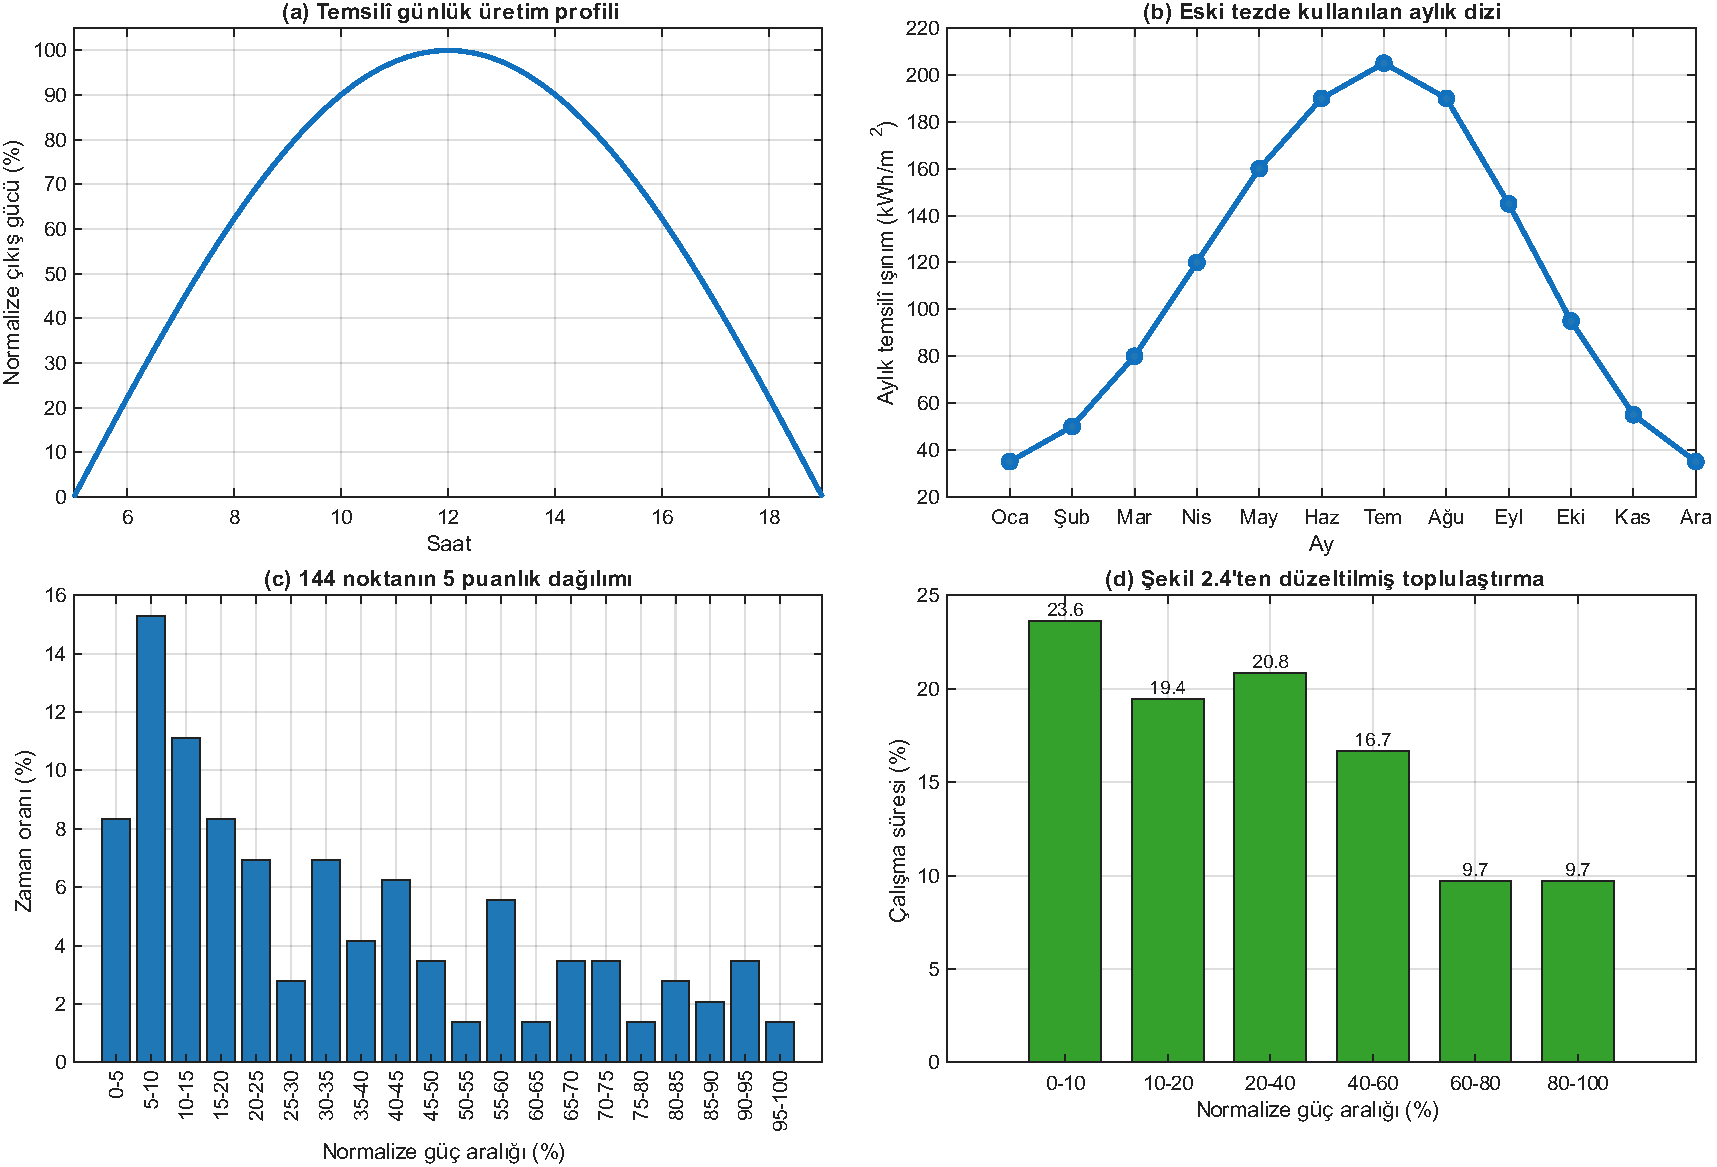
\includegraphics[width=\textwidth]{literatur/matlab_b2_guc_profilleri.pdf}
  \caption{Temsilî günlük ve aylık FV profilleri ile 144 çalışma noktasının MATLAB'da üretilen güç dağılımı. (d) paneli, (c) panelindeki nokta sayılarının güç sınıflarına yeniden gruplanmasıyla elde edilmiştir.}
  \label{fig:fv-calisma-profilleri}
\end{figure}

Günlük ve aylık diziler arasındaki çarpım bağı şu şekilde tanımlanmıştır. Saat indisi $h$, ay indisi $m$, boyutsuz gün içi normalize profil $p_d(h)$ ve aya bağlı temsilî ışınım seviyesi $G_m(m)$ ile gösterilsin. Aynı birimi $G_m$'den alan temsilî yıl--saat ışınımı $G_{\mathrm{tem}}(m,h)$
\begin{equation}
G_{\mathrm{tem}}(m,h)=G_m(m)\,p_d(h)
\label{eq:temsili-yil-saat-yuzeyi}
\end{equation}
biçiminde tanımlanır. Eşitlik~\eqref{eq:temsili-yil-saat-yuzeyi} ölçülmüş bir saha modeli değil, iki normalize dizinin çarpımıdır. Fotovoltaik gücün ışınımla orantılı olduğu basitleştirilmiş kabul altında $P_{\mathrm{tem}}(m,h)/P_n\approx G_{\mathrm{tem}}(m,h)/G_{\max}$ bağıntısı elde edilir; burada $P_{\mathrm{tem}}$ temsilî gücü, $P_n$ anma gücünü ve $G_{\max}$ yüzeydeki en büyük ışınımı gösterir. Temsilî örneklemdeki yaklaşık \SI{4}{\watt\per\metre\squared} ve \SI{200}{\watt\per\metre\squared} uçları, 50 katlık bir çalışma aralığına ve en düşük sıfırdan farklı noktanın tepe değerin yaklaşık \SI{2}{\percent}'sine karşılık geldiğine işaret etmektedir.

Şekil~\ref{fig:fv-calisma-profilleri}(c)'deki sayımlar 144 temsilî çalışma noktasına karşılık gelmektedir. İlk iki güç sınıfında toplam 34 nokta bulunması, eşit ağırlıklı ay--saat örneklemi içindeki noktaların \SI{23.6}{\percent}'sının anma gücünün \SI{10}{\percent}'undan düşük olduğunu gösterir. \SI{23.6}{\percent} oranı gerçek yıllık çalışma süresini değil, kullanılan temsilî örnekleme düzeninin dağılımını ifade etmektedir. Üç yıllık saha verisine dayanan bir çalışma, ışınımın önemli bir bölümünün düşük ve orta seviyelerde gerçekleştiğini; düşük ışınım ile evirici eşik kayıplarının sistem performansını etkilediğini göstermiştir \citep{Mondol2007}. Farklı iklim koşullarında yürütülen ağırlıklı verim incelemesi de yalnızca tepe veriminin saha davranışını temsil etmeye yetmediğini, evirici performansının değişen ışınım ve kısmi yük seviyeleriyle birlikte değerlendirilmesi gerektiğini ortaya koymuştur \citep{AbRahman2020}. Sonuç olarak \SI{23.6}{\percent} değeri evrensel bir yıllık oran olarak değil, düşük güç bölgesinin incelenmesini motive eden temsilî örneklem sonucu olarak kullanılmaktadır.

\begin{table}[htbp]
  \centering
  \caption{Temsilî 144 çalışma noktasının güç sınıfı dağılımı.}
  \label{tab:fv-guc-dagilimi}
  \begin{tabular}{ccc}
    \toprule
    \textbf{Çıkış gücü ($\%P_n$)} & \textbf{Nokta sayısı} & \textbf{Temsilî oran (\%)} \\
    \midrule
    0--10 & 34 & 23,6 \\
    10--20 & 28 & 19,4 \\
    20--40 & 30 & 20,8 \\
    40--60 & 24 & 16,7 \\
    60--80 & 14 & 9,7 \\
    80--100 & 14 & 9,7 \\
    \midrule
    Toplam & 144 & 100,0 \\
    \bottomrule
  \end{tabular}
\end{table}

Yıllık enerji verimi yalnızca tepe verimle belirlenmediğinden Avrupa ve CEC ağırlıklı verim tanımları, farklı yük noktalarındaki dönüşüm verimlerini belirli katsayılarla birleştirir. Alt indis $x$, anma gücünün yüzde $x$ noktasını; $\eta_x$ ise aynı noktadaki dönüşüm verimini göstersin. Avrupa ağırlıklı verimi
\begin{equation}
\eta_{\mathrm{EU}}=0{,}03\eta_{5}+0{,}06\eta_{10}+0{,}13\eta_{20}+0{,}10\eta_{30}+0{,}48\eta_{50}+0{,}20\eta_{100}
\label{eq:eta-eu}
\end{equation}
ve CEC ağırlıklı verimi
\begin{equation}
\eta_{\mathrm{CEC}}=0{,}04\eta_{10}+0{,}05\eta_{20}+0{,}12\eta_{30}+0{,}21\eta_{50}+0{,}53\eta_{75}+0{,}05\eta_{100}
\label{eq:eta-cec}
\end{equation}
olarak tanımlanır \citep{Sera2008,Sandia2015}. Eşitlik~\eqref{eq:eta-eu} ve Eşitlik~\eqref{eq:eta-cec} içindeki katsayıların toplamı birdir; iki ifade de boyutsuz ağırlıklı ortalamadır. Deneysel test düzenekleri ve standartlaştırılmış protokoller, verimin güç seviyesi, giriş gerilimi ve MPPT koşullarıyla birlikte ölçülmesini öngörür \citep{Sera2008,Sandia2015}. İzmir ışınım verilerine dayalı çalışma da bölgesel güç dağılımının ağırlık katsayılarını değiştirebildiğini göstermiştir \citep{Ongun2013}.

\begin{table}[htbp]
  \centering
  \caption{Avrupa ve CEC ağırlıklı verim katsayıları \citep{Sera2008,Sandia2015}.}
  \label{tab:agirlikli-verim-katsayilari}
  \begin{tabular}{c*{6}{c}}
    \toprule
    \textbf{Yöntem} & \multicolumn{6}{c}{\textbf{Güç seviyesi ve ağırlık katsayısı}} \\
    \midrule
    Avrupa & $5:0{,}03$ & $10:0{,}06$ & $20:0{,}13$ & $30:0{,}10$ & $50:0{,}48$ & $100:0{,}20$ \\
    CEC & $10:0{,}04$ & $20:0{,}05$ & $30:0{,}12$ & $50:0{,}21$ & $75:0{,}53$ & $100:0{,}05$ \\
    \bottomrule
  \end{tabular}
\end{table}

Kısmi yük davranışının verim ve harmonik boyutları Şekil~\ref{fig:fv-verim-thd-profilleri} üzerinde birlikte verilmiştir. Paneller (a) ve (c) genel eğilimi gösteren tipik dizilerdir; belirli bir ürünün doğrulanmış veri sayfası veya yeni deney sonucu değildir. Paneller (b) ve (d) aynı dizilerin 144 temsilî çalışma noktasına uygulanmasından elde edilen ikincil hesaplardır ve tez katkısının performans kanıtı olarak kullanılmamaktadır.

\begin{figure}[H]
  \centering
  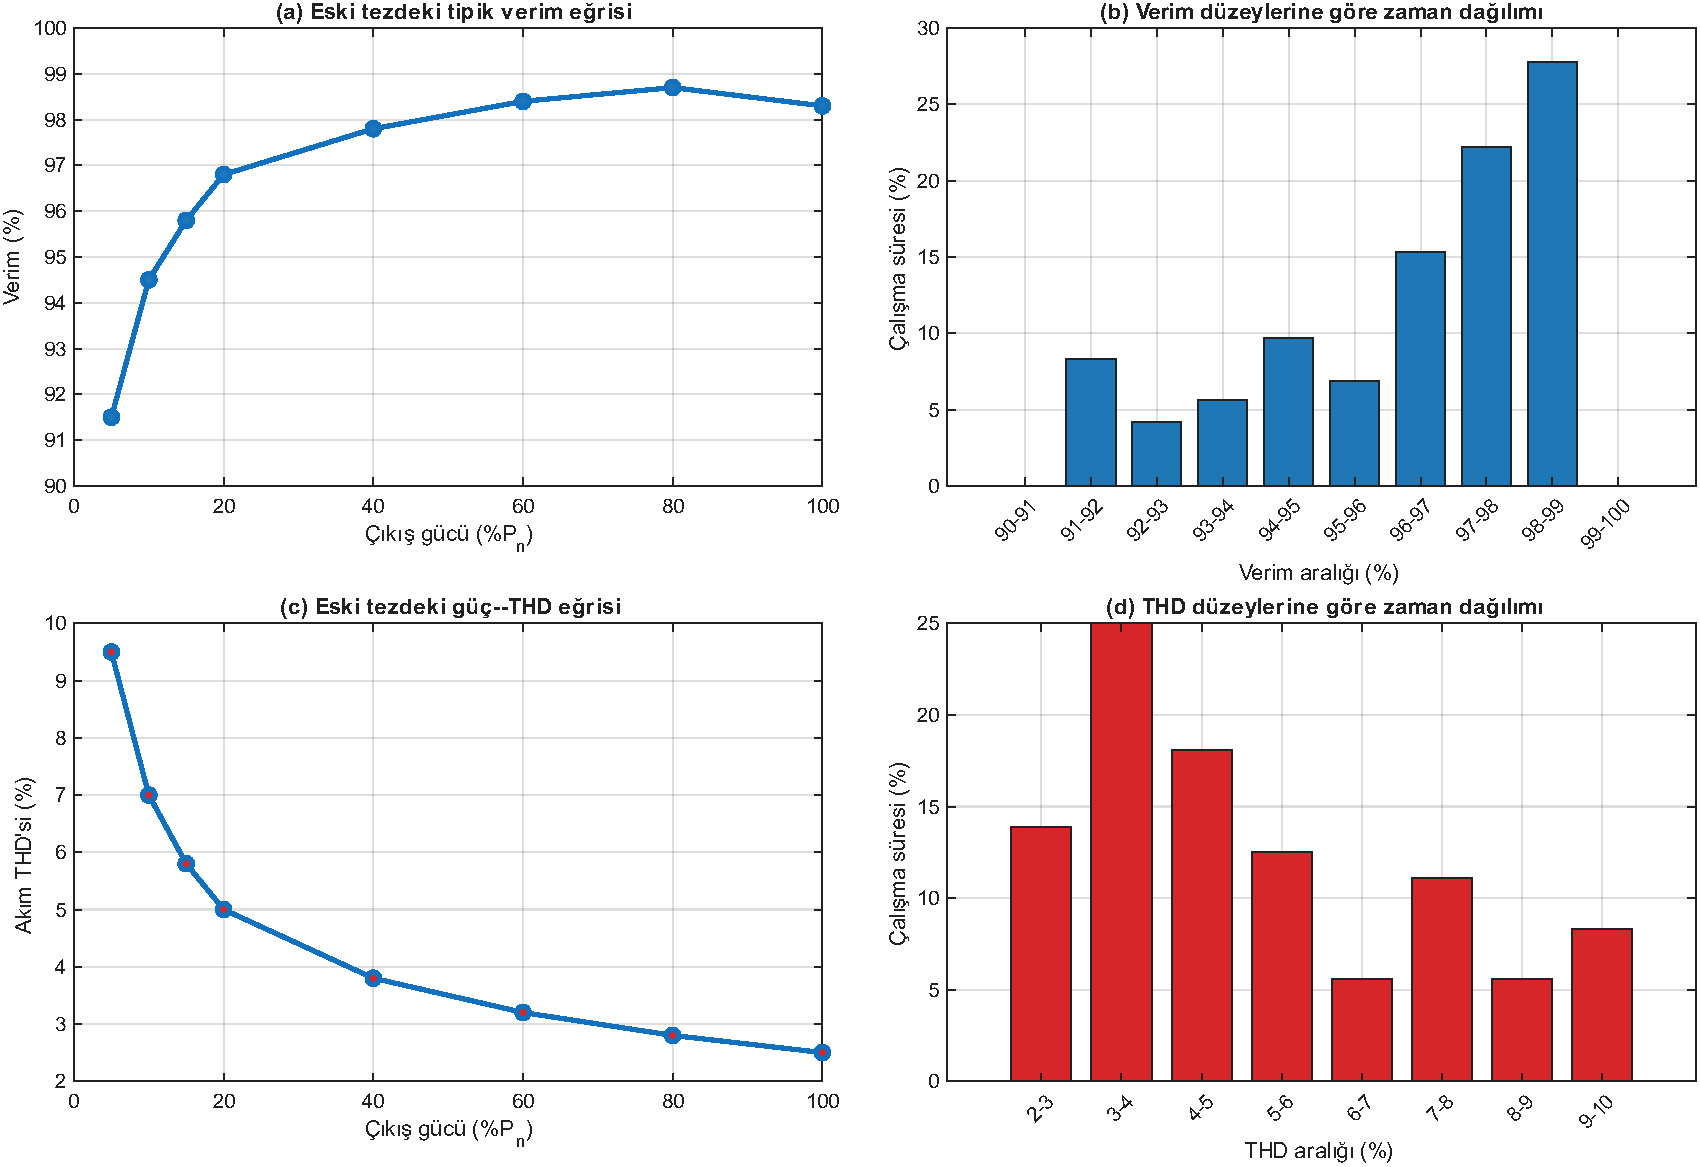
\includegraphics[width=\textwidth]{literatur/matlab_b2_verim_thd_profilleri.pdf}
  \caption{Tipik kısmi yük verim ve THD eğrileri ile bunlardan türetilen temsilî zaman dağılımlarının MATLAB'da vektörel üretimi.}
  \label{fig:fv-verim-thd-profilleri}
\end{figure}

Şekil~\ref{fig:fv-verim-thd-profilleri}(a)'daki dizide verim, \SI{5}{\percent} yükte yaklaşık \SI{91.5}{\percent}, \SI{10}{\percent} yükte \SI{94.5}{\percent} ve \SI{80}{\percent} yükte \SI{98.7}{\percent} düzeyindedir. Aynı şeklin (c) panelinde akım THD'si \SI{5}{\percent} yükte \SI{9.5}{\percent}, \SI{20}{\percent} yükte \SI{5.0}{\percent} ve anma gücünde \SI{2.5}{\percent} olarak verilmiştir. Şeklin bölümdeki amacı, yalnızca tepe veriminin ve anma gücündeki THD'nin yıllık davranışı açıklamaya yetmediğini ortaya koymaktır.

Düşük güçte THD artışının dış literatür kanıtı, \citet{Chicco2009} tarafından raporlanan günlük güç ve akım THD kaydıyla Şekil~\ref{fig:chicco-guc-thd} üzerinde gösterilmiştir. Sabah ve akşam düşük güç bölgelerinde THD'nin yükselmesi, tezin kısmi yük odağını destekler; belirli harmoniklerin T-tipi nötr kol mekanizmasından kaynaklandığını tek başına kanıtlamaz.

\begin{figure}[H]
  \centering
  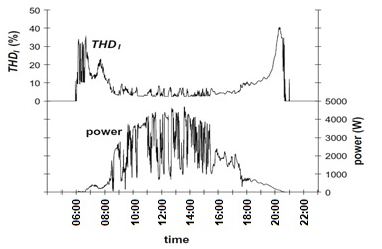
\includegraphics[width=0.62\textwidth]{literatur/chicco2009_guc_thd.png}
  \caption{\SI{5}{\kilo\watt} sınıfındaki bir FV eviricinin gün içi çıkış gücü ve akım THD'si; \citet{Chicco2009}'dan alınmıştır.}
  \label{fig:chicco-guc-thd}
\end{figure}

Şebekeye bağlı \SI{10}{\kilo\watt} sınıfındaki ticari bir eviricinin sabah devreye giriş kaydı Tablo~\ref{tab:ticari-evirici-thd} üzerinde verilmiştir. Cihaz seri numarası, güç analizörü, örnekleme penceresi, şebeke gerilimi ve ham dosya mevcut olmadığından satırlar yeni deney kanıtı değil, düşük güç bölgesinin önemini gösteren ve ham kaydı belgelenmemiş bir gözlem kaydıdır.

\begin{table}[H]
  \centering
  \caption{Ticari bir eviricinin sabah devreye girişinde kaydedilen güç ve akım THD değerleri; ham ölçüm dosyası ve protokolü belgelenmemiş motivasyon kaydı.}
  \label{tab:ticari-evirici-thd}
  \begin{tabular}{lrrr}
    \toprule
    \textbf{Zaman} & \textbf{Güç (W)} & \textbf{Güç ($\%P_n$)} & \textbf{THD (\%)} \\
    \midrule
    Devreye ilk giriş & 100 & 1,00 & 400 \\
    07:50 & 500 & 5,00 & 34 \\
    08:00 & 580 & 5,80 & 27 \\
    08:10 & 729 & 7,29 & 26 \\
    08:35 & 1060 & 10,60 & 17 \\
    08:50 & 1320 & 13,20 & 14 \\
    09:05 & 1450 & 14,50 & 14 \\
    09:18 & 1720 & 17,20 & 13 \\
    09:26 & 1880 & 18,80 & 9 \\
    09:42 & 2200 & 22,00 & 8 \\
    \bottomrule
  \end{tabular}
\end{table}

\begin{figure}[H]
  \centering
  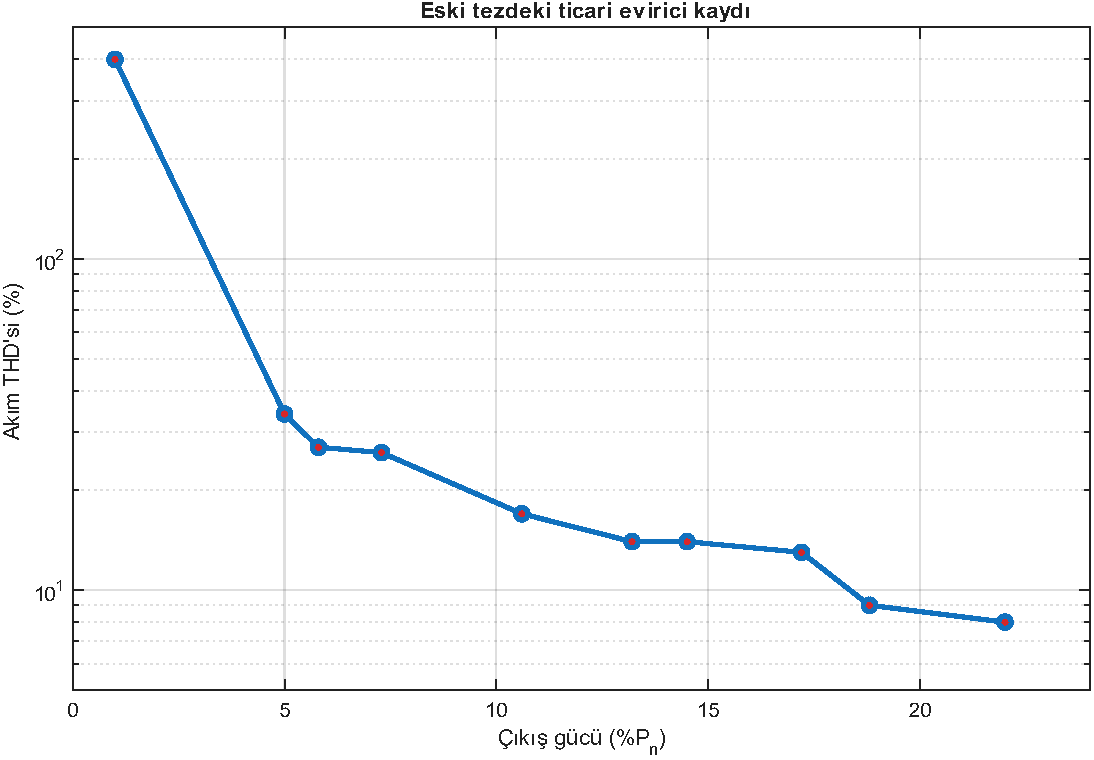
\includegraphics[width=0.84\textwidth]{literatur/matlab_b2_ticari_evirici_thd.pdf}
  \caption{Tablo~\ref{tab:ticari-evirici-thd}'deki kaydın MATLAB'da çizimi; düşey eksen logaritmiktir; veri, ham kaydı belgelenmemiş motivasyon kaydıdır.}
  \label{fig:ticari-evirici-thd}
\end{figure}

Şekil~\ref{fig:ticari-evirici-thd}, kayıttaki doğrusal olmayan azalmayı logaritmik eksende görünür hâle getirmektedir: akım THD'si anma gücünün \SI{1}{\percent}'inde \SI{400}{\percent} iken \SI{22}{\percent}'sinde \SI{8}{\percent} düzeyine iner. Grafiğin bölümdeki görevi, devreye giriş ve düşük güç test noktalarının yalnızca anma gücündeki tek bir ölçümle temsil edilemeyeceğini göstermektir; ham kaydı belgelenmemiş bir gözlem olarak önerilen anahtarlama yönteminin başarısını kanıtlamaz, laboratuvar deneylerinin düşük güç noktasında yürütülmesini gerekçelendirir.

Temsilî FV profili ile ticari evirici kaydının tezdeki rolü motivasyonla sınırlıdır. Şekil~\ref{fig:fv-calisma-profilleri} ve Tablo~\ref{tab:fv-guc-dagilimi} belirli bir konum için sorgulanmış PVGIS ham çıktısına, Tablo~\ref{tab:ticari-evirici-thd} ise cihaz modeli, analizör ve ölçüm penceresi belgelenmiş bir ham kayda dayanmamaktadır. İki içerik, düşük güç bölgesinin işletmede sık görüldüğünü ve düşük güçte akım THD'sinin yükseldiğini literatürle birlikte nitel olarak destekler; tezin verim ve THD bulgularına sayısal girdi oluşturmaz. Saha profili ve ham kayıt eksikliği Bölüm~\ref{chap:sonuc} içinde sınırlılık olarak yer almaktadır.

Düşük güçte sürücü, kontrol, anahtarlama ve manyetik elemanların güce zayıf bağlı kayıpları toplam çıkışa oranla büyür. Şebeke akımının küçük olması, ölü zaman ve anahtar doğrusal olmayanlıklarının temel bileşene oranını da artırır. Saha ve laboratuvar ölçümleri, FV eviricilerde akım dalga biçimi bozulmasının güç seviyesi ve şebeke gerilim kalitesiyle değiştiğini göstermektedir \citep{Kjaer2005,Chicco2009}. Harmonik sınırları bağlantı gücü ve standart kapsamına göre tanımlansa da yalnızca toplam THD değerine bakılması, hangi harmonik bileşenin hangi fiziksel mekanizmadan kaynaklandığını açıklamaz \citep{IEC61000}.

Ters akım problemi, senkron alçaltıcı dönüştürücünün hafif yük davranışı üzerinden açıklanabilir. Sürekli iletim kipinde (Continuous Conduction Mode, CCM) alt anahtar akım sıfırı geçtikten sonra açık tutulursa endüktör akımı negatif yönde büyür ve kaynak ile yük arasında yararlı güç üretmeyen enerji dolaşımı oluşur. Diyot benzetimi veya süreksiz iletim kipinde (Discontinuous Conduction Mode, DCM) senkron anahtar akım sıfıra yaklaşırken kapatılarak negatif akım engellenir \citep{Erickson2001,Mohan2003}. Chen ve arkadaşları, hafif yükte diyot benzetimi ile sürekli iletim kipini kayıp bileşenleri bakımından karşılaştırmış; ters akımın engellenmesinin RMS akımı ve iletim kaybını azaltabildiğini, ancak anahtarın ideal olmayan sıfır akım algılama anının yeni kayıplar oluşturabileceğini göstermiştir \citep{Chen2010}.

Diyot benzetimi ile sürekli iletim kipindeki endüktör akımları Şekil~\ref{fig:de-ccm-akim} üzerinde karşılaştırılmıştır. Sürekli iletim kipindeki akımın sıfırın altına geçmesi, tezde nötr anahtar üzerinden oluşan ters akımın açıklanmasında kullanılan temel benzerliği oluşturmaktadır.

\begin{figure}[htbp]
  \centering
  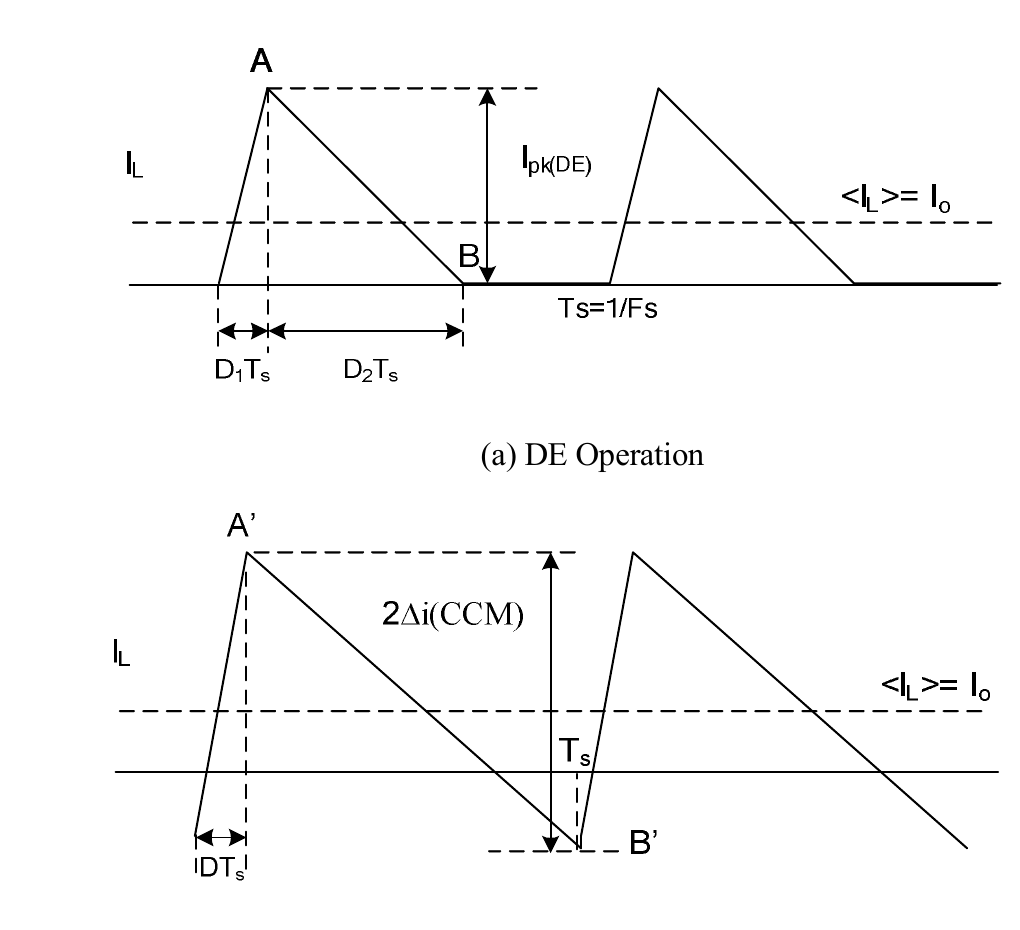
\includegraphics[width=0.68\textwidth]{literatur/gecici_de_ccm_akim_chen34.png}
  \caption{Diyot benzetimi (DE) ve sürekli iletim (CCM) kiplerinde endüktör akımının karşılaştırılması; Chen ve arkadaşlarından alınmıştır \citep{Chen2010}.}
  \label{fig:de-ccm-akim}
\end{figure}

Şebekeye bağlı T-tipi eviricide sıfır gerilim durumunu oluşturan nötr kol, akımın işaret değiştirmesine izin verdiğinde benzer bir senkron alçaltıcı davranışı gösterebilir. Nötr anahtarın susturulması ters akım yolunu keserken faz düğümünün doğal diyot yolları üzerinden farklı bir gerilim durumuna geçmesine neden olur. Kayıp azalması ile anahtarlama darbe dizisinin değişmesi böylece aynı fiziksel müdahalenin iki sonucudur. Literatürdeki genel süreksiz iletim bilgisi ters akımı açıklamak için gerekli kuramsal temeli sağlasa da T-tipi faz kolunda oluşan gerilim hatasının üçüncü harmonik etkisini ve şebeke akım kontrolüyle etkileşimini tek başına açıklamamaktadır.

Senkron alçaltıcıdaki CCM/DCM ayrımının T-tipi nötr kol üzerindeki karşılığı, tezin benzetim modelinden aynı zaman tabanında üretilmiştir. Nötr anahtar susturmada $Q_1$--$Q_4$ kapı komutları Şekil~\ref{fig:s2-kapi-isaretleri} üzerinde, klasik anahtarlama ile susturmanın kutup gerilimi ve şebeke akımı Şekil~\ref{fig:s1-s2-kalibre-dalga} üzerinde verilmiştir. Susturmalı çalışmada $L_1$ akımı söndüğünde kutup gerilimi üç seviyeden hiçbirinde bulunmaz; sürmesiz aralık, Şekil~\ref{fig:de-ccm-akim} içindeki diyot benzetimi kipinin sıfır akım aralığına karşılık gelir. $L_1$ akımının her anahtarlama çevriminde sıfıra oturduğu aralıklar Şekil~\ref{fig:susturma-l1-yakin} üzerinde, sürmesiz aralığın zaman oranı ve köprü davranışına etkisi Kesim~\ref{sec:dusuk-akim-modelleme} içinde gösterilmiştir.

\section{Şebeke Akım Kontrolü ve İleri Besleme Yaklaşımları}

Düşük güç mekanizması tek başına devre düzeyinde çözülemez; ters akımı kesen her müdahale, akım kontrol döngüsünün gördüğü bitkiyi de değiştirir. Kesim, tezin kompanzasyon katkısının dayandığı kontrol literatürünü özetlemektedir. Şebekeye bağlı bir eviricide akım denetleyicisi, referans akım ile ölçülen akım arasındaki hatadan modülasyon gerilimi üretir. Senkron referans çerçevesi, durağan eksen PI kontrolü ve oransal-rezonans (Proportional-Resonant, PR) kontrolü yaygın seçenekler arasındadır. PR denetleyici, temel frekansta yüksek kazanç sağlayarak sinüzoidal referansın kalıcı durum hatasını azaltabilir; seçili harmoniklerde ek rezonans kolları da kullanılabilir \citep{Teodorescu2006PR,Teodorescu2011}. Faz kilitlemeli döngü (Phase-Locked Loop, PLL) veya eşdeğer bir eşzamanlama yapısı, şebeke faz ve frekans bilgisini üretir; tek fazlı sistemlerde ortogonal işaret üretimi ve dijital gecikmeler tasarımın parçasıdır \citep{Blaabjerg2006,Zhou2018}.

LCL filtre, daha küçük toplam endüktansla yüksek frekanslı anahtarlama bileşenlerini zayıflatabilmesine karşılık rezonans tepesi oluşturur. Pasif sönümleme direnç kaybı doğururken aktif sönümleme ölçülen akım veya gerilim işaretlerinden sanal empedans etkisi üretir. PR denetleyici ile LCL aktif sönümlemenin birlikte tasarımı, kapalı çevrim kutupları ve kararlılık marjları dikkate alınarak yapılmalıdır \citep{Zhang2014PR}. Şebeke gerilimi ileri beslemesi, ortak bağlantı noktasındaki bozucu gerilimin akıma taşınmasını azaltmak için modülasyon girişine ölçülen gerilimden türetilen bir terim ekler. Lu ve arkadaşları, dijital gecikmenin ileri besleme yolunu LCL rezonansı üzerinde aktif sönümleme veya negatif sönümleme üretebilen dinamik bir elemana dönüştürebildiğini göstermiştir \citep{Lu2016}. Zayıf şebeke koşullarını inceleyen Wang ve arkadaşları da şebeke empedansına bağlı pozitif geri besleme etkisinin faz marjını azaltabileceğini ve ileri besleme kanalının frekans seçici biçimde tasarlanması gerektiğini ortaya koymuştur \citep{Wang2024}.

Anahtar ölü zamanı, snubber ve parazitik kapasiteler de komut edilen gerilim ile gerçekleşen faz gerilimi arasında akım yönüne bağlı hata oluşturur. Zhang ve Xu, parazitik kapasitelerin anahtarlama kenarlarını sonlu eğimli hâle getirdiğini ve klasik darbe tabanlı ölü zaman kompanzasyonunun özellikle küçük akımlarda yetersiz kalabildiğini deneysel olarak göstermiştir \citep{Zhang2014Deadtime}. Düşük güç harmonikleri, yalnızca denetleyici bant genişliğinin değil; modülasyon, anahtar geçişi, akım yönü ve şebeke geriliminin ortak sonucudur.

Sin\textsuperscript{3} tabanlı yaklaşımın literatürdeki yerini doğru kurabilmek için üçüncü harmonik enjeksiyonu ile bozucu bastırma amaçlı ileri besleme ayrılmalıdır. Klasik üçüncü harmonik enjeksiyonu, faz referanslarına ortak mod bileşeni ekleyerek DA bara kullanım oranını artırmayı veya belirli anahtarlama harmoniklerini düzenlemeyi hedefler \citep{Holmes2003,Aghdam2013}. Tezde ele alınan Sin\textsuperscript{3} terimi ise nötr anahtar susturma yönteminin oluşturduğu üçüncü harmonik etkisine karşı, ölçülen şebeke işaretinden $\sin^3(\theta)=[3\sin(\theta)-\sin(3\theta)]/4$ özdeşliğiyle üretilen bir şekillendirme bileşenidir. Fourier gösterimi matematiksel temeli sağlarken terimin modülasyon girişine eklenmesi onu hata sinyalinden türetilen bağımsız bir geri besleme denetleyicisi yapmaz \citep{Oppenheim1997}.

İdeal doğrusal ve doyumsuz modelde dışsal ileri besleme terimi kapalı çevrimin karakteristik paydasını değiştirmeyebilir. Gerçek dönüştürücüde örnekleme, PWM gecikmesi, LCL rezonansı, sınırlayıcılar ve çalışma noktasına bağlı anahtarlama doğrusal olmayanlıkları ideal ayrımı sınırlar. Periyodik çalışma noktaları çevresindeki frekans bağlaşımının incelenmesi gerektiğinde doğrusal zamanla periyodik modeller ve harmonik transfer fonksiyonları (Harmonic Transfer Function, HTF) kullanılabilir \citep{Wereley1991,Liao2022}. Tez açısından temel gereksinim, Sin\textsuperscript{3} teriminin kontrolcü olarak adlandırılması değil; mevcut akım döngüsündeki konumunun, kapalı çevrim aktarımının ve düşük ile anma gücü koşullarındaki etkisinin açıkça doğrulanmasıdır.

\section{Literatürün Karşılaştırmalı Değerlendirilmesi}

Dört bilgi alanının tezin araştırma sorularıyla kesişimi Tablo~\ref{tab:literatur-karsilastirma} üzerinde toplanmıştır. Tablo, tezin üç katkı ekseniyle en yakından ilişkili çalışmaları kullanılan yapı, temel amaç, doğrulama düzeyi ve tez açısından kalan sınır üzerinden karşılaştırmaktadır; bir çalışmanın genel başarısını değil, tezin araştırma sorularını ne ölçüde kapsadığını gösterir.

\begin{longtable}{>{\raggedright\arraybackslash}p{0.18\textwidth} >{\raggedright\arraybackslash}p{0.20\textwidth} >{\raggedright\arraybackslash}p{0.24\textwidth} >{\raggedright\arraybackslash}p{0.26\textwidth}}
\caption{Tezle doğrudan ilişkili çalışmaların karşılaştırmalı sentezi.}\label{tab:literatur-karsilastirma}\\
\toprule
\textbf{Çalışma} & \textbf{Yapı ve odak} & \textbf{Doğrulama} & \textbf{Tez açısından kalan sınır} \\
\midrule
\endfirsthead
\caption[]{Tezle doğrudan ilişkili çalışmaların karşılaştırmalı sentezi (devamı).}\\
\toprule
\textbf{Çalışma} & \textbf{Yapı ve odak} & \textbf{Doğrulama} & \textbf{Tez açısından kalan sınır} \\
\midrule
\endhead
\bottomrule
\endfoot
Schweizer ve Kolar \citep{Schweizer2013} & Üç seviyeli T-tipi dönüştürücü; kayıp ve verim & Analitik kayıp hesabı ve donanım prototipi & Düşük güçte nötr kol ters akımı ve ters akıma bağlı THD ele alınmamıştır. \\
Wang ve ark. \citep{Wang2020} & \SI{250}{\kilo\watt} SiC T-tipi evirici; güç yoğunluğu ve geçiş kayıpları & Kayıp modeli ve tam ölçekli prototip & Çalışma çekiş eviricisine ve yüksek güç tasarımına odaklanmıştır. \\
Chen ve ark. \citep{Chen2010} & Senkron buck; diyot benzetimi ve sürekli iletim & Analiz, benzetim ve deney & T-tipi şebeke eviricisinin sıfır durumu ve harmonik sonucu kapsanmamıştır. \\
Zhang ve Xu \citep{Zhang2014Deadtime} & Ölü zaman ve parazitik kapasite kompanzasyonu & Darbe modeli ve deney & Nötr anahtar susturma kaynaklı üçüncü harmonik hedeflenmemiştir. \\
Lu ve ark. \citep{Lu2016} & LCL eviricide şebeke gerilimi ileri beslemesi & Frekans alanı analizi ve deney & Sin\textsuperscript{3} tabanlı anlık şekillendirme ve düşük güç ters akımı ele alınmamıştır. \\
Wang ve ark. \citep{Wang2024} & Zayıf şebekede filtreli ileri besleme & Empedans modeli ve yarı fiziksel benzetim & Amaç şebeke empedansına uyumdur; anahtarlama kaynaklı üçüncü harmonik değildir. \\
Momayyezan ve ark. \citep{Momayyezan2016} & Yeniden yapılandırılabilir yüksek gerilim batarya dönüştürücüsü & Beş modüllü ölçekli prototip & Şebekeye bağlı üç seviyeli T-tipi evirici ve düşük güç yöntemiyle bütünleşmemiştir. \\
Farakhor ve ark. \citep{Farakhor2023} & Modüler yeniden yapılandırılabilir BESS ve hücre gücü yönetimi & Optimizasyon, benzetim ve laboratuvar prototipi & T-tipi/Vienna işlev paylaşımı ve şebeke akımı kalitesi hedeflenmemiştir. \\
Huang ve ark. \citep{Huang2024} & Anahtar tabanlı modüler yeniden yapılandırma ve dengeleme & Kayıp analizi ve ölçekli deney & İlaveli modül anahtarları kullanılmış; ortak T-tipi güç katı ele alınmamıştır. \\
\end{longtable}

\section{Araştırma Boşluğu}

Literatür taraması üç ayrı bilgi kümesinin gelişmiş olduğunu göstermektedir. İlk küme, T-tipi dönüştürücünün yüksek verim, güç yoğunluğu, anahtarlama geçişleri ve elektromanyetik uyumluluk özelliklerini açıklamaktadır \citep{Schweizer2013,Wang2020,Hizarci2021}. İkinci küme, hafif yükte ters akımı azaltan süreksiz iletim veya diyot benzetimi ilkelerini ve şebeke eviricilerindeki harmonik/ileri besleme problemlerini ele almaktadır \citep{Chen2010,Lu2016,Wang2024}. Üçüncü küme ise batarya modüllerini veya dönüştürücü elemanlarını farklı çalışma kiplerinde yeniden kullanan EDS mimarilerini geliştirmektedir \citep{Momayyezan2016,Farakhor2023,Huang2024}.

Kümeler arasındaki bağlantı sınırlıdır. T-tipi eviricinin düşük güçte sıfır durumunu oluşturan nötr kolun senkron buck benzeri ters akım mekanizması, aynı müdahalenin verim ve üçüncü harmonik üzerindeki karşıt etkileriyle birlikte yeterince incelenmemiştir. Ters akımı kesen anahtarlama değişikliği ile oluşan harmonik bileşeni, mevcut kapalı çevrimi bağımsız bir denetleyiciyle değiştirmeden şekillendiren Sin\textsuperscript{3} tabanlı ileri besleme terimi için de doğrudan bir karşılık belirlenememiştir. Yeniden yapılandırılabilir batarya literatürü işlev paylaşımının mümkün olduğunu gösterse de T-tipi evirici, Vienna PFC ve aktif batarya yönetimi işlevlerinin aynı yarı iletken yapı üzerinde birleştirilmesi; düşük güç anahtarlama ve şebeke akımı kalitesi ekseniyle ortak bir tez çerçevesinde ele alınmamıştır.

Belirlenen araştırma boşluğu, üç katkıyı tek bir sav altında birleştirmektedir: T-tipi dönüştürücünün anahtarlama durumları düşük güçte ters akımı azaltacak biçimde yeniden düzenlenebilir; ortaya çıkan harmonik ödünleşimi Sin\textsuperscript{3} tabanlı ileri besleme kompanzasyonuyla yönetilebilir; aynı topolojinin yarı iletkenleri EDS'nin farklı şarj--deşarj ve dengeleme kiplerinde yeniden görevlendirilebilir. Sonraki bölümlerde tezin savı; ortak sistem modeli, çalışma kipleri, elektriksel parametreler, kapalı çevrim analizleri ve erişilebilir benzetim/deney kanıtı üzerinden sınanacaktır.
